\setLTR
$a: 0xAC620014$

$b: 0x0082082A$
\setRTL

\subsubsection*{الف}
در این باید کد اسمبلی معادل با هر دستور را بنویسیم. برای این کار ابتدا اعداد را به باینری تبدیل می‌کنیم:
\setLTR

$a=(10101100011000100000000000010100)_2$

$b=(00000000100000100000100000101010)_2$

\setRTL

حال از این تصویر استفاده کرده و دستورات را شناسایی می‌کنیم:

\setLTR
\qquad\qquad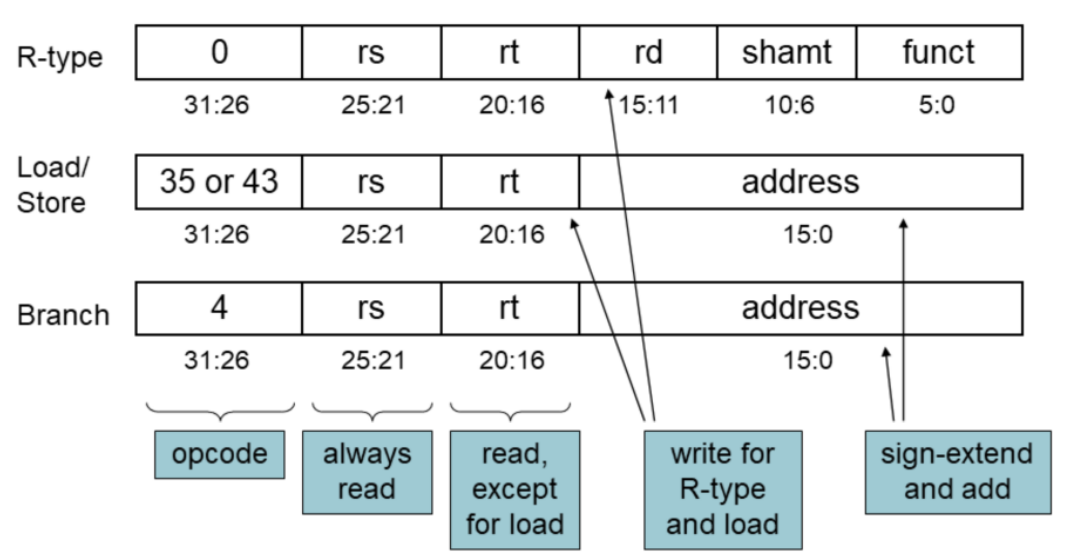
\includegraphics[scale=0.5]{figs/1.png}

$opcode_a = a[31:26] = (101011)_2 = (43)_{10} \longrightarrow store$

$
\begin{cases}
	r_s = a[25:21] = (00011)_2 = (3)_{10} \longrightarrow v_1 \\ 
	r_t = a[20:16] = (00010)_2 = (2)_{10} \longrightarrow v_0 \\
	immediate = a[15:0] = (0000000000010100)_2 = (20)_{10}
\end{cases}\longrightarrow
sw \ \ \$v_0 , 20(\$v_1)
$\\ \\ \\

$opcode_b = b[31:26] = (000000)_2 = (0)_{10} \longrightarrow R-Type$

$
\begin{cases}
	r_s = b[25:21] = (00100)_2 = (4)_{10} \longrightarrow a_0 \\ 
	r_t = b[20:16] = (00010)_2 = (2)_{10} \longrightarrow v_0 \\
	r_d = b[15:11] = (00001)_2 = (1)_{10} \longrightarrow a_t \\
	function = b[5:0] = (101010)_2 \longrightarrow set \ on \ less \ than 
\end{cases} \qquad \longrightarrow
slt \ \ \$a_t \ ,\ \$a_0 \ , \ \$v_0
$\\ \\ \\
\setRTL

\subsubsection*{ب}
خروجی extend sign دستور a ، 16 بیت اول دستور را به یک عدد 32 بیتی تبدیل می‌کند با حفظ علامت:
\setLTR

$output=(00000000000000000000000000010100)_2 = (14)_{16}$

\setRTL

خروجی واحد left shift که توسط دستور b اجرای می‌شود، خروجی واحد extend sign را می‌گیرد و 2 بیت به چپ شیفت می‌دهد.
\setLTR

$output = (010000010000010000010101000)_2 = (20820A8)_{16}$

\setRTL

\subsubsection*{ج}

در این بخش باید مقادیر واحد کنترل ALU را به ازای هر دستور محسابه کنیم. از تصویر زیر کمک می‌گیریم:

\setLTR
\qquad\qquad\qquad\qquad\qquad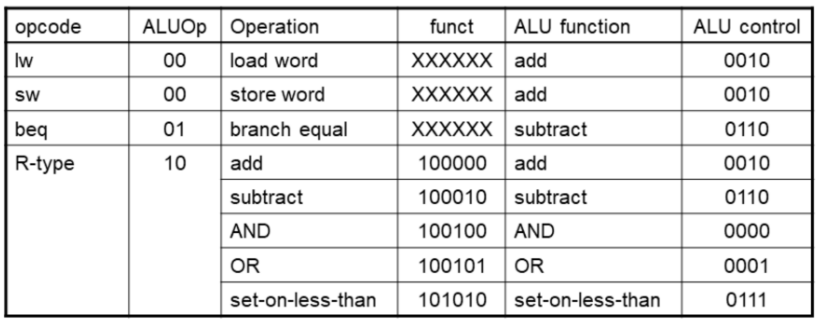
\includegraphics[scale=0.45]{figs/2.png}

$
a\rightarrow lw \rightarrow \begin{cases}
ALUOp = 00 \\
funct =  a[5:0] = \times
\end{cases}
$

$
b\rightarrow R Type \rightarrow \begin{cases}
	ALUOp = 10 \\
	funct = b[5:0] = 101010
\end{cases}
$

\setRTL

\subsubsection*{د}

با توجه به این‌که هیچ کدام از دستورات مربوط به دستورات jump و یا branch نیستند، پس در هر دو حالت مقدار برابر است با:

\setLTR

$PC \leftarrow PC + 4$

\setRTL

در شکل زیر مسیرهایی که از آن‌ها این مقادیر به‌دست می‌آیند را می‌بینید:

\setLTR
\qquad\qquad\qquad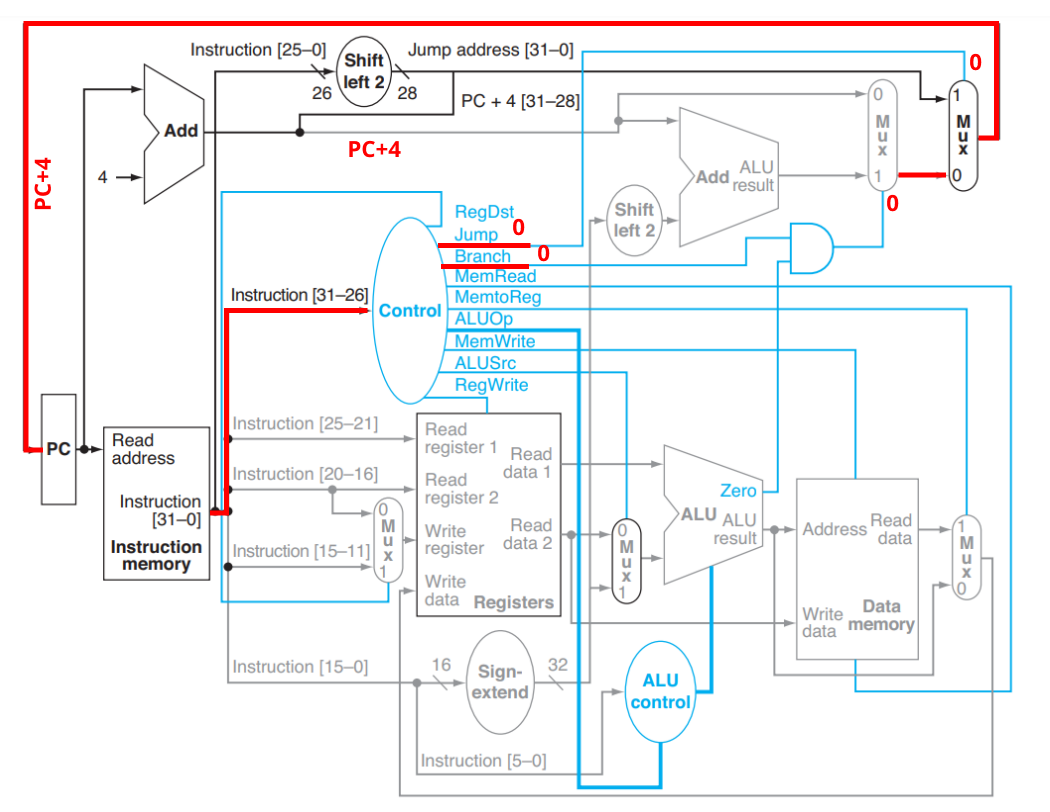
\includegraphics[scale=0.29]{figs/3.png}

\setRTL

\subsubsection*{ه}

